% 4th-iso.tex

\documentclass[tikz]{standalone}
\usetikzlibrary{positioning, decorations.pathreplacing}

\begin{document}
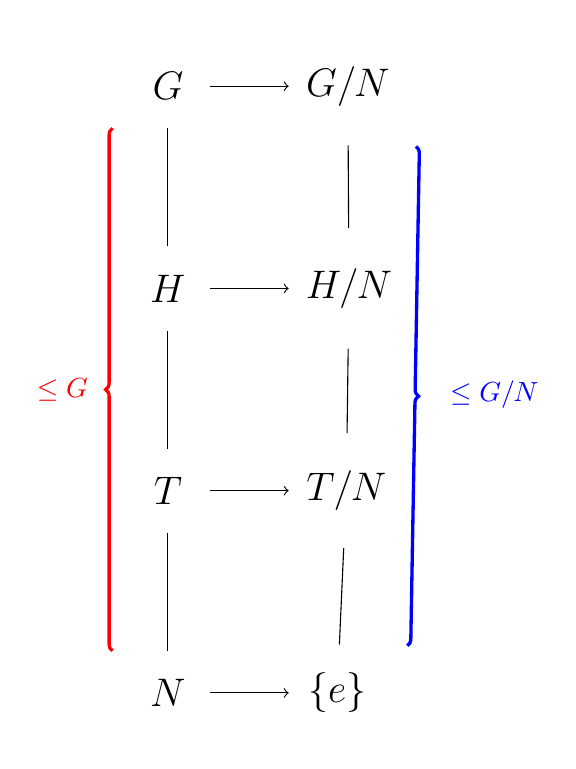
\begin{tikzpicture}[group/.style = {circle, minimum size = 30pt, font = \Large},
  node distance = 1.5cm and 1.0cm]
  \node (g) [group] {$G$};
  \node (h) [group, below = of g] {$H$};
  \node (t) [group, below = of h] {$T$};
  \node (n) [group, below = of t] {$N$};
  \path (g) edge[] (h)
		(h) edge[] (t)
		(t) edge[] (n);

  \node (g1) [group, right = of g] {$G/N$};
  \node (h1) [group, right = of h] {$H/N$};
  \node (t1) [group, right = of t] {$T/N$};
  \node (n1) [group, right = of n] {$\{e\}$};
  \path (g1) edge[] (h1)
		(h1) edge[] (t1)
		(t1) edge[] (n1);

  \foreach \i in {g, h, t, n} {
	\draw [->] (\i) to (\i1);
  }

  \draw[very thick, decoration = {brace, mirror, raise = 20pt}, decorate, red] (g) to node[left = 25pt] {$\le G$} (n);
  \draw[very thick, decoration = {brace, raise = 25pt}, decorate, blue] (g1) to node[right = 35pt] {$\le G/N$} (n1);
\end{tikzpicture}
\end{document}
